\chapter{Empirical Comparison of Learning Algorithms}\label{ch:comparison}
In this chapter, we provide an empirical evaluation of the learning algorithms
described in Chapter~\ref{ch:structured_pystruct}.  We use the open source
implementations in \pystruct, and publish the evaluation code and datasets with
the package.

\section{Datasets and Models}
We consider several qualitatively different datasets, that have been widely used in the literature.
The problems we consider are multi-class classification, sequence labeling, multi-label prediction,
and general graph labeling.

\subsection{Multi-Class Classification (MNIST)}
\begin{figure}
    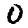
\includegraphics[width=.092\linewidth, frame]{evaluation/images/mnist_digit_0}
    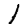
\includegraphics[width=.092\linewidth, frame]{evaluation/images/mnist_digit_1}
    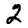
\includegraphics[width=.092\linewidth, frame]{evaluation/images/mnist_digit_2}
    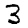
\includegraphics[width=.092\linewidth, frame]{evaluation/images/mnist_digit_3}
    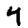
\includegraphics[width=.092\linewidth, frame]{evaluation/images/mnist_digit_4}
    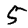
\includegraphics[width=.092\linewidth, frame]{evaluation/images/mnist_digit_5}
    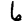
\includegraphics[width=.092\linewidth, frame]{evaluation/images/mnist_digit_6}
    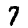
\includegraphics[width=.092\linewidth, frame]{evaluation/images/mnist_digit_7}
    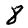
\includegraphics[width=.092\linewidth, frame]{evaluation/images/mnist_digit_8}
    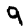
\includegraphics[width=.092\linewidth, frame]{evaluation/images/mnist_digit_9}
    \caption{%
        Visualization of samples from the ten classes in the MNIST dataset.\figlabel{mnist_illustration}
    }
\end{figure}
The simplest task we use is multi-class classification. In this task,
the inference problem is trivial, as it is assumed the target set is small enough
to be enumerated efficiently. While this problem could be solved more efficiently
with specialized algorithms, it nevertheless provides an initial insight into structured
prediction algoriths.
We choose the classical MNIST dataset of handwritten digits, consisting of
60000 training images and 10000 test images of the digits zero to nine.
\Figref{mnist_illustration} shows some examples. Each image is a $28 \times 28$
grey-level image, resulting in a $784$-dimensional feature vector. We normalize
the feature to lie between $0$ and $1$.
%
\enlargethispage{15mm}
The model we use for multi-class classification is the Crammer-Singer
formulation. We do not include a bias, leading to $784 \cdot 10 = 7840$
parameters in the model.


\begin{figure}
    
\includegraphics[width=.068\linewidth, frame]{evaluation/images/justifications_00}
    
\includegraphics[width=.068\linewidth, frame]{evaluation/images/justifications_01}
    
\includegraphics[width=.068\linewidth, frame]{evaluation/images/justifications_02}
    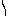
\includegraphics[width=.068\linewidth, frame]{evaluation/images/justifications_03}
    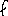
\includegraphics[width=.068\linewidth, frame]{evaluation/images/justifications_04}
    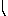
\includegraphics[width=.068\linewidth, frame]{evaluation/images/justifications_05}
    
\includegraphics[width=.068\linewidth, frame]{evaluation/images/justifications_06}
    
\includegraphics[width=.068\linewidth, frame]{evaluation/images/justifications_07}
    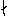
\includegraphics[width=.068\linewidth, frame]{evaluation/images/justifications_08}
    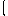
\includegraphics[width=.068\linewidth, frame]{evaluation/images/justifications_09}
    
\includegraphics[width=.068\linewidth, frame]{evaluation/images/justifications_10}
    
\includegraphics[width=.068\linewidth, frame]{evaluation/images/justifications_11}
    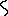
\includegraphics[width=.068\linewidth, frame]{evaluation/images/justifications_12}\\[3mm]
    
\includegraphics[width=.068\linewidth, frame]{evaluation/images/skiing_00}
    
\includegraphics[width=.068\linewidth, frame]{evaluation/images/skiing_01}
    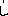
\includegraphics[width=.068\linewidth, frame]{evaluation/images/skiing_02}
    
\includegraphics[width=.068\linewidth, frame]{evaluation/images/skiing_03}
    
\includegraphics[width=.068\linewidth, frame]{evaluation/images/skiing_04}\\[3mm]
    
\includegraphics[width=.068\linewidth, frame]{evaluation/images/unexpected_00}
    
\includegraphics[width=.068\linewidth, frame]{evaluation/images/unexpected_01}
    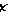
\includegraphics[width=.068\linewidth, frame]{evaluation/images/unexpected_02}
    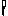
\includegraphics[width=.068\linewidth, frame]{evaluation/images/unexpected_03}
    
\includegraphics[width=.068\linewidth, frame]{evaluation/images/unexpected_04}
    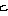
\includegraphics[width=.068\linewidth, frame]{evaluation/images/unexpected_05}
    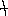
\includegraphics[width=.068\linewidth, frame]{evaluation/images/unexpected_06}
    
\includegraphics[width=.068\linewidth, frame]{evaluation/images/unexpected_07}
    
\includegraphics[width=.068\linewidth, frame]{evaluation/images/unexpected_08}\\
    \caption{%
        Visualization of some words from the OCR dataset. The first letters were removed by \citet{taskar2003max} as 
        they were capitals.
        The words are: (j)ustifications, (s)kiing and (u)nexpected. The letters in parentheses are not part of the dataset.
        \figlabel{ocr_illustration}
    }
\end{figure}
\subsection{Sequence Labeling (OCR)}
A classical application of structured prediction is sequence labeling.
We choose the ``OCR'' dataset introduced in the seminal work of \citet{taskar2003max}.
Each input consists of the segmented handwritten letters of a word in lower
case. The task is to classify all letters in a word, that is assign each
segmented input letter one of the classes ``a'' to ``z''. As the first letter
of each word was capitalized, these were removed by \citet{taskar2003max},
leading to somewhat odd-looking labels. The words are between three and fourteen
letters long, and each letter is represented as a binary image of size $16
\time 8$, with a toal of $6877$ words.
The dataset is devided into ten folds. We consider two setups: learning
on one fold, and testing on the remaining nine folds, following \citet{taskar2003max},
and learning on nine folds and testing on the remaining fold, following \citet{lacoste}.
We refer to the learning on one fold as OCR-small, and learning on nine folds as OCR-big.
We use a simple chain model with a single constant pairwise feature.
This means the unary potential has $16 \cdot 8 \cdot 26$ parameters, one for each input
feature and output class. The pairwise potential consists of a matrix of
transition potentials with $26 \cdot 26=676$ entries.
It is well-known that efficient exact inference in chains is possible using
message passing algorithms. 


\subsection{Multi-Label Classification}
Multi-label classification is a generalization of multi-class classification,
in which each example can be associated with more than one class. In other
words, the algorihm must decide for each sample and for each class whether the
sample belongs to that class or not.
Multi-label classification was first formulated as a structured prediction problem
in by \citet{finley2008training}, where it was used to investigate the influence of
approximate inference on the $n$-slack cutting plane algorithm. In this formulation,
each class is represented as a binary node in a factor graph---the states representing
presence of absence of the class. A different factor of pairwise potentials is introduced
between each pair of classes.
We also consider a different model, where pairwise potentials are only
introduced between specific nodes. Build a tree over the binary variables by
computing the Chow-Liu Tree~\citep{chow1968approximating} of the targets. While
this results in a less expressive model, a tree-shaped model allows for exact
inference via message passing.
We use two of the datasets used in \citet{finley2008training}, the scene
and yeast datasets. We choose these two as these are real-world datasets for
which the pairwise approach outlined above actually improves upon the
baseline~\citep{finley2008training}.
The scene dataset has six labels, 294 input features, 1211 training samples and
1196 test samples. This leads to $204 \cdot 6$ parameters for the unary potentials,
$3 \cdot 5 \cdot 4$ parameters for the full pairwise potentials (four for each edge), and
$5 \cdot 4$ parameters for the pairwise potentials of the tree-shaped model.
Using four parameters for each edge is a slight over-parametrization that
simplifies writing out the model.
The yeast dataset has 14 labels, 103 features, 1500 training samples and 971
test samples. The resulting numbers of parameters are $14 \cdot 103$ parameters
for the unary potentials, $7 \cdot 13 \cdot 4$ parameters for the full pairwise
potential, and $13 \cdot 4$ parameters for the tree-shaped model.

\begin{figure}
    \begin{tabu} to \linewidth{@{}XXXXXXX@{}}
    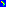
\includegraphics[width=\linewidth]{evaluation/images/snake_input_0001}&%
    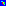
\includegraphics[width=\linewidth]{evaluation/images/snake_input_0002}&%
    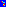
\includegraphics[width=\linewidth]{evaluation/images/snake_input_0003}&%
    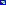
\includegraphics[width=\linewidth]{evaluation/images/snake_input_0004}&%
    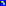
\includegraphics[width=\linewidth]{evaluation/images/snake_input_0005}&%
    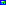
\includegraphics[width=\linewidth]{evaluation/images/snake_input_0006}&%
    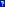
\includegraphics[width=\linewidth]{evaluation/images/snake_input_0007}\\
    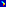
\includegraphics[width=\linewidth]{evaluation/images/snake_label_0001}&%
    
\includegraphics[width=\linewidth]{evaluation/images/snake_label_0002}&%
    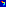
\includegraphics[width=\linewidth]{evaluation/images/snake_label_0003}&%
    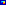
\includegraphics[width=\linewidth]{evaluation/images/snake_label_0004}&%
    
\includegraphics[width=\linewidth]{evaluation/images/snake_label_0005}&%
    
\includegraphics[width=\linewidth]{evaluation/images/snake_label_0006}&%
    \includegraphics[width=\linewidth]{evaluation/images/snake_label_0007}
    \end{tabu}
\caption{%
    Visualization of the snakes dataset. The top row shows input patterns, the bottom row the corresponding
    labels. The colors in the image showing the labels correspond to dark blue for background, and encoding
    the length of the snake from head (red) to tail (blue).
\figlabel{snakes_illustration}}
\end{figure}

\subsection{2D Grid CRF (Snakes)}
The snakes dataset is a synthetic dataset, where samples are labeld 2D grids.
It was introduced in \citet{nowozin2011decision} to demonstrate the importance
of learning conditional pairwise potentials. The dataset consists of ``snakes''
of length ten traversing the 2D grid. Each grid cell that was visited is marked
as the snake heading out towards the top, bottom, left, or right, while
unvisited cells are marked as background.  The goal is to predict a labeling of
the snake from ``head'' to ``tail'', that is assigning numbers from zero to
nine to the cells that are occupied by the snake.  \Figref{snakes_illustration} illustrates the
principle.
Local evidence for the target label is weak except
around head and tail, making this a challenging task. Pairwise potentials are necessary to solve the
task. The dataset is noise-free in the sense that given the above description, a
human could easily produce the desired labeling without making any mistake.
The dataset is also interesting as the model of \citet{nowozin2011decision} produced
notoriously hard to optimize energy functions.

In \citet{nowozin2011decision}, the input was encoded into five RGB colors
(``up'', ``down'', ``left'', ``right'', ``background'').  To encode the input
more suitable for our linear methods, we convert this representation to a
one-hot encoding of the five states.

We use a grid CRF model for this task. Unary for each node are given by the
input of the 8-neighborhood of the node---using a 4-neighborhood would most
likely yield better results, but we do not want to encode too much
task-knowledge into our model.
Using the one-hot encoding of the input, this leads to $9 \dot 5 = 45$ unary features.
With 11 output classes, the unary potential has $11 \cdot 9 \cdot 5$ parameters.
Features for the pairwise potentials are constructed by concatenating the features
of the two neighboring nodes, taking the direction of the edge into account.
The pairwise feature therefore has dimensionality $45 \cdot 4$, with the first
$45$ entries corresponding to the feature of the ``top'' node, the second $45$
entries to the features ``bottom'' node, followed bye the ``left'' and
``right'' nodes. As each edge is either horizontal \emph{or} vertical, only two
of these parts will be non-zero for any given edge.  With $45 \cdot 4$ edge
features, the pairwise potentials has $45 \cdot 4 \cdot 11^2$ parameters.


\subsection{Superpixel CRFs for Semantic Segmentation}
Our main attention is devoted to the use of conditional random fields for
semantic segmentation.  We use the Pascal VOC and MSRC datasets. A detailed
description of the method will be given in Chapter~\ref{ch:exact_learning}.
%TODO will it?
The Pascal VOC has \ldots training and \ldots test images, each having
around 100 superpixels. There are 20 object categories, plus background. The % TODO check!
MSRC dataset has \ldots training and \ldots test images, also segmented in
around 100 superpixels each. We use the MSRC-21 dataset, which has 21 target
classes.
Each superpixel is represented as an output variable, with the ground truth obtained
by majority vote over the pixel belonging to the superpixel.
Pairwise potentials were introduced for each pair of neighboring superpixels.
We then removed all superpixels that were labeled as ``void'', together with
their pairwise potentials.
As unary potentials, we use the TextonBoost probabilities provided by \citet{krahenbuhl2012efficient}.
We average probabilities inside each superpixel, yielding 21 input features for both datasets.
We also used the same pairwise features for the two datasets: a constant feature,
a color contrast feature, and a feature encoding relative vertical position between superpixels.
Overall, the models for both datasets had $21 \cdot 21 + 21^2 \cdot 4$ features.
It is possible to assume symmetric potentials for this dataset, leading to less
pairwise features. We found both parametrizations yielded similar results.

\begin{table}
    \caption{Summary of Datasets.\tablabel{datasets}}
    \begin{tabu} to \linewidth{@{}XXXXXX@{}}
    %\multicolumn{2}{@{}c@{}}{\includegraphics[width=\linewidth]{evaluation/legend.pdf}}\\
    \toprule
    Dataset    & samples & nodes & edges & dim w & labels\\
    \cmidrule{1-6}
    MNIST      & 60000   & 1     & none  &       & 10\\
    OCR-small  & 704     & 3--14 & chain &       & 26\\
    OCR-large  & 6173    & 3--14 & chain &       & 26\\
    scene-tree & 1211    & 6     & tree  &       & 2\\
    scene-full & 1211    & 6     & loopy &       & 2\\
    yeast-tree & 1500    & 14    & tree  &       & 2\\
    yeast-full & 1500    & 14    & loopy &       & 2\\
    snake      & 200     &84--168& loopy &       & 11\\
    MSRC21     & 276     & 7--113& loopy &       & 21\\
    Pascal VOC & 964     & 8--112& loopy &       & 21\\
    \bottomrule

    \end{tabu}
\end{table}

\section{Experiments}
We compare the following algorithms on the above models:
\begin{itemize}
    \item Stochastic Subgradient Descent using the Pegasos schedule: %TODO
    %\item Stochastic Subgradient Descent using the Pegasos schedule: AVERAGING
    \item The $1$-slack cutting plane algorithm without constraint caching.
    \item The $1$-slack cutting plane algorithm with constraint caching. For
            each sample, the last $50$ inference results are stored.
            Details of the caching strategy can be found in Chapter~\ref{ch:exact_learning}.
            %TODO
    \item The $n$-slack cutting plane algorithm, where the QP is solved after each training.
    \item The $n$-slack cutting plane algorithm, where the QP is solved every 100 training samples.
    \item The SZLJSP algorithm.
\end{itemize}
All algorithm take a $C$ parameter, which we adjusted on a fully trained model
on a validation set (experiments not reported here) and held constant for all models.
We found, however, that the algorithms and models are quite robust to the choice of $C$ within
one or two orders of magnitude.
As stopping criterion, we used a duality gap of $0.1$ when possible, and a
pre-defined number of iterations for the subgradient algorithms. It is worth
noting that the quadratic programming based algorithms have additional
hyper-parameters that we do not discuss here in detail, such as the threshold
for removing a constraint as inactive, how often inactive constraints are
removed, and parameters of the underlying QP solver. On the other hand, the
SZLJSP, for example, has no hyper-parameters except for the stopping criterion.

Our ultimate evaluation criterion is how fast the learning algorithms converge,
and how robust they are to approximate inference.  To quantify our goals, we
track primal suboptimality and training set error during learning, as well as
final error on the test set.
We report suboptimality as a function of runtime, and as a function of passes
over the training set.  Both are important to practitioners, as they give
important insight into the workins of the algorithm.  The actual runtime is
certainly the most important factor, but also highly influenced by
implementation details and properties of the dataset. We are particularly
interested in cases where inference is highly non-trivial, making inference the
dominating factor of runtime.
We define one pass over the dataset as calling prediction once for each sample.
This way, we can get a clear picture how learning times with complexity of the
inference task. For the subgradient and SZLJSP algorithms, learning time is linear
in the number of passes ofver the dataset, while chaching and solving of a QP makes
the learning time depend on the number of iterations in hard-to-predict ways.

\subsection{Experiments using Exact Inference}
In this section, we present results on multi-class classification, sequence
labeling and multi-label prediction with a tree-structured model. In these
tasks, exact inference is possible, and we can compute the exact objective of
the various algorithms easily. We use the dynamic programming algorithm
implemented in \textsc{OpenGM} for experiments.

We start our experiments with the MNIST dataset.
The convergence of the primal objective and training set loss in terms of
passes over the training set is shown in \Figref{mnist_iterations}.
Several trends can be observed: the $n$-slack cutting plane algorithms are converge fastest, with
the version that recomputes the QP at every step leading the race. The algorithms are
closely followed by the caching $1$-slack cutting plane algorithm.
They are followed by the significantly slower SZLJSP algorithm, and finally
the non-caching $1$-slack cutting plane algorithm and subgradient descent.
These results are intiutive, as they reflect ``how much work'' each algorithm does
for each loss-augmented prediction step. More work towards the objective leads to faster convergence.
This ``more work'' is quantified in \Figref{mnist_times}.
Clearly the $1$-slack algorithms to ``to much'' work, leading to very slow
convergence.  Also, caching does not speed up learing learning on this dataset,
as loss-augmented predction is as fast as querying the cache.

\begin{figure}
    \begin{tabu} to \linewidth{@{}XX@{}}
    \multicolumn{2}{@{}c@{}}{\includegraphics[width=\linewidth]{evaluation/legend.pdf}}\\[-3mm]
    \includegraphics[width=\linewidth]{evaluation/images/letters_small_log}&%
    \includegraphics[width=\linewidth]{evaluation/images/letters_small_log_time}
    \end{tabu}
\caption{%
   Convergence of the primal objective on OCR-small. 
\figlabel{ocr_small_results}}
\end{figure}

We now consider datasets with non-trivial inference.
The results for OCR-small are shown in \Figref{ocr_small_results}.
The trends seen in the figures are similar to what we saw for MNIST above.
Again, even though inference is non-trivial, the non-caching $1$-slack
algorithm is slower than the caching one. Again, the plots against passes over the trainingset
do not reflect the runtime complexity of the $n$-slack approach.

\begin{figure}
    \begin{center}
    \includegraphics[width=.5\linewidth]{evaluation/images/letters_small_dual}
\end{center}
\caption{%
   Convergence of the primal objective on OCR-small. 
\figlabel{ocr_small_dual}}
\end{figure}

There is one interesting phenomenon to be seen here: The cutting-plane algorithms stop immediately
when reaching the desired suboptimality of $0.1$. The SZLJSP algorithm, on the other hand, keeps
on learning much longer---even longer than it took to get to the desired suboptimality. This is caused
by a much looser bound given by the dual. Remember that the stopping criterion for both cutting-plane 
and SZLJSP are given by the duality gap. It seems that while the primal objective converges much
faster in the SZLJSP algorithm than in the non-caching $1$-slack algorithm, the dual does not.
This means that in for this practical experiment, the non-caching $1$-slack algorithm was \emph{faster}
in guaranteeing the desired suboptimality.
\Figref{ocr_small_dual} illustrates this point by ploting primal and dual
objectives for the $1$-slack cutting plane and the SZLJSP algorithms.

\begin{figure}
    \begin{tabu} to \linewidth{@{}XX@{}}
    \multicolumn{2}{@{}c@{}}{\includegraphics[width=\linewidth]{evaluation/legend.pdf}}\\[-3mm]
    \includegraphics[width=\linewidth]{evaluation/images/letters_big_log}&%
    \includegraphics[width=\linewidth]{evaluation/images/letters_big_log_time}
    \end{tabu}
\caption{%
   Convergence of the primal objective on OCR-large. 
\figlabel{ocr_large_results}}
\end{figure}

The results for the OCR-large dataset are shown in \Figref{ocr_large_results}
The trends are the same as for the smaller dataset: $n$-slack and caching $1$-slack cutting plane are very fast
in terms of passes through the dataset, but $n$-slack cutting plane is impractical slow
with respect to runtime. The SZLJSP algorithm converges fast intially, but the $1$-slack cutting plane
is faster at high precision and faster in certifying the desired duality gap.
%TODO initially 1-slack is beaten by ssgd

\begin{figure}
    \begin{tabu} to \linewidth{@{}XX@{}}
    \multicolumn{2}{@{}c@{}}{\includegraphics[width=\linewidth]{evaluation/legend.pdf}}\\[-3mm]
    \includegraphics[width=\linewidth]{evaluation/images/scene_tree_log}&%
    \includegraphics[width=\linewidth]{evaluation/images/scene_tree_log_time}\\
    \includegraphics[width=\linewidth]{evaluation/images/scene_full_log}&%
    \includegraphics[width=\linewidth]{evaluation/images/scene_full_log_time}\\
    \includegraphics[width=\linewidth]{evaluation/images/yeast_tree_log}&%
    \includegraphics[width=\linewidth]{evaluation/images/yeast_tree_log_time}
    \end{tabu}
\caption{%
   Convergence of the primal objective on the multi-label datasets. From top to
   bottom: the scene dataset using a tree model, the scene dataset using a full
   model, the yeast dataset using a tree model, and the yeast dataset using a
   full model.
\figlabel{multi-label-results}}
\end{figure}

Next, we consider the multi-label task, starting with the tree-shaped models.
The results for the yeast and scene datasets are shown in \Figref{yeast_tree} and \Figref{scene_tree},
respectively. The caching $1$-slack algorithm is much faster than the non-caching one on both datasets.
The caching $1$-slack algorithm is the fastest algorithm to achieve the desired primal suboptimality.
On the scene dataset, the other cutting-plane base algorithms are second fastest, while they
lag behind the stoachastic algorithms on the larger yeast dataset. Again, initial convergence is
faster for the stochastic algorithms.

The results when using the full model are shown in \Figref{yeast_full} and \Figref{scene_full}.
Here, inference is much more complex than in the previous tasks.

\subsection{Experiments using Approximate Inference}
For the remaining tasks of multi-label classification with the full graph, the
snakes dataset and image segmentation, exact inference is usually not possible.

We use two different approximate inference algorithms, fusion moves, a fast
local search procedure, and AD$^3$, a dual-subgradient method to solve the LP
relaxation of the inference problem.
Evaluation of algorithms where exact inference is not possible is much harder,
as it is usually not possible to evaluate the exact objective. When using AD$^3$,
we can still consider the relaxed task, which will be solved exactly in the
majority of cases (AD$^3$ sometimes fails to find the primal solution to the LP
relaxation). %TODO is this happening?
When using fusion moves, there is no obvious interpretation of the produced
primal objective, other than that it provides a lower bound of the actual
objective. Nevertheless, we find it informative to analyze the behavior of this lower bound.

For both inference algorithms, we also evaluate the predictive performance on
the training set.  We explicitly do not consider the relaxed problem
here---instead we round possible fractional results.
While the training error does not directly reflect the objective, it provides
a measure of how effective the ``prediction machine'' given by the learned model
together with the inference algorithm is.

\section{Discussion}
From the experiments above, it is clear there is currently \emph{no single best algorithm}.
We can say, however, that the stochastic subgradient descent algorithm with
pegasos step-size always converged slower, both in terms of learning time and
in passes over the dataset, as the SZLJSP algorithm.
Together with the fact that stochastic subgradient descent has no good stopping
criterion, there seems to be no reason to use the stochastic gradient descent.
